\documentclass{article}
\usepackage{amsmath}
\usepackage{amsfonts}
\usepackage{tikz}
\usepackage{qtree}
\usetikzlibrary{automata,arrows}

\begin{document}

\section*{Student Information}
Name: Batuhan Akçan \\
ID: 2580181 \\

\section*{Answer 1}
i: 1954\\
ii: Enigma\\
iii: Turing test\\
iv: The Chemical Basis of Morphogenesis\\
v: The Imitation Game

\section*{Answer 2}
\subsection*{a)}
$M = (K, \Sigma, \delta, s, H)$ where\\
$K = \{q_0, q_1, q_2, q_3, y\}$,\\
$\Sigma = \{a,b,\sqcup,\triangleright\}$,\\
$s = q_0$,\\
$H = \{y\}$,\\
$\delta$ is:\\
$\delta(q_0,a) = (q_0,\rightarrow)$,\\
$\delta(q_0,b) = (q_1,\rightarrow)$,\\
$\delta(q_0,\triangleright) = (q_0,\rightarrow)$,\\
$\delta(q_0,\sqcup) = (q_3,\rightarrow)$,\\
$\delta(q_1,a) = (q_1,\rightarrow)$,\\
$\delta(q_1,b) = (q_2,\rightarrow)$,\\
$\delta(q_1,\triangleright) = (q_1,\rightarrow)$,\\
$\delta(q_1,\sqcup) = (q_3,\rightarrow)$,\\
$\delta(q_2,a) = (q_3,\rightarrow)$,\\
$\delta(q_2,b) = (q_3,\rightarrow)$,\\
$\delta(q_2,\triangleright) = (q_2,\rightarrow)$,\\
$\delta(q_2,\sqcup) = (y,\sqcup)$,\\
$\delta(q_3,a) = (q_3,\rightarrow)$,\\
$\delta(q_3,b) = (q_3,\rightarrow)$,\\
$\delta(q_3,\triangleright) = (q_3,\rightarrow)$,\\
$\delta(q_3,\sqcup) = (q_3,\rightarrow).$\\
\subsection*{b)}
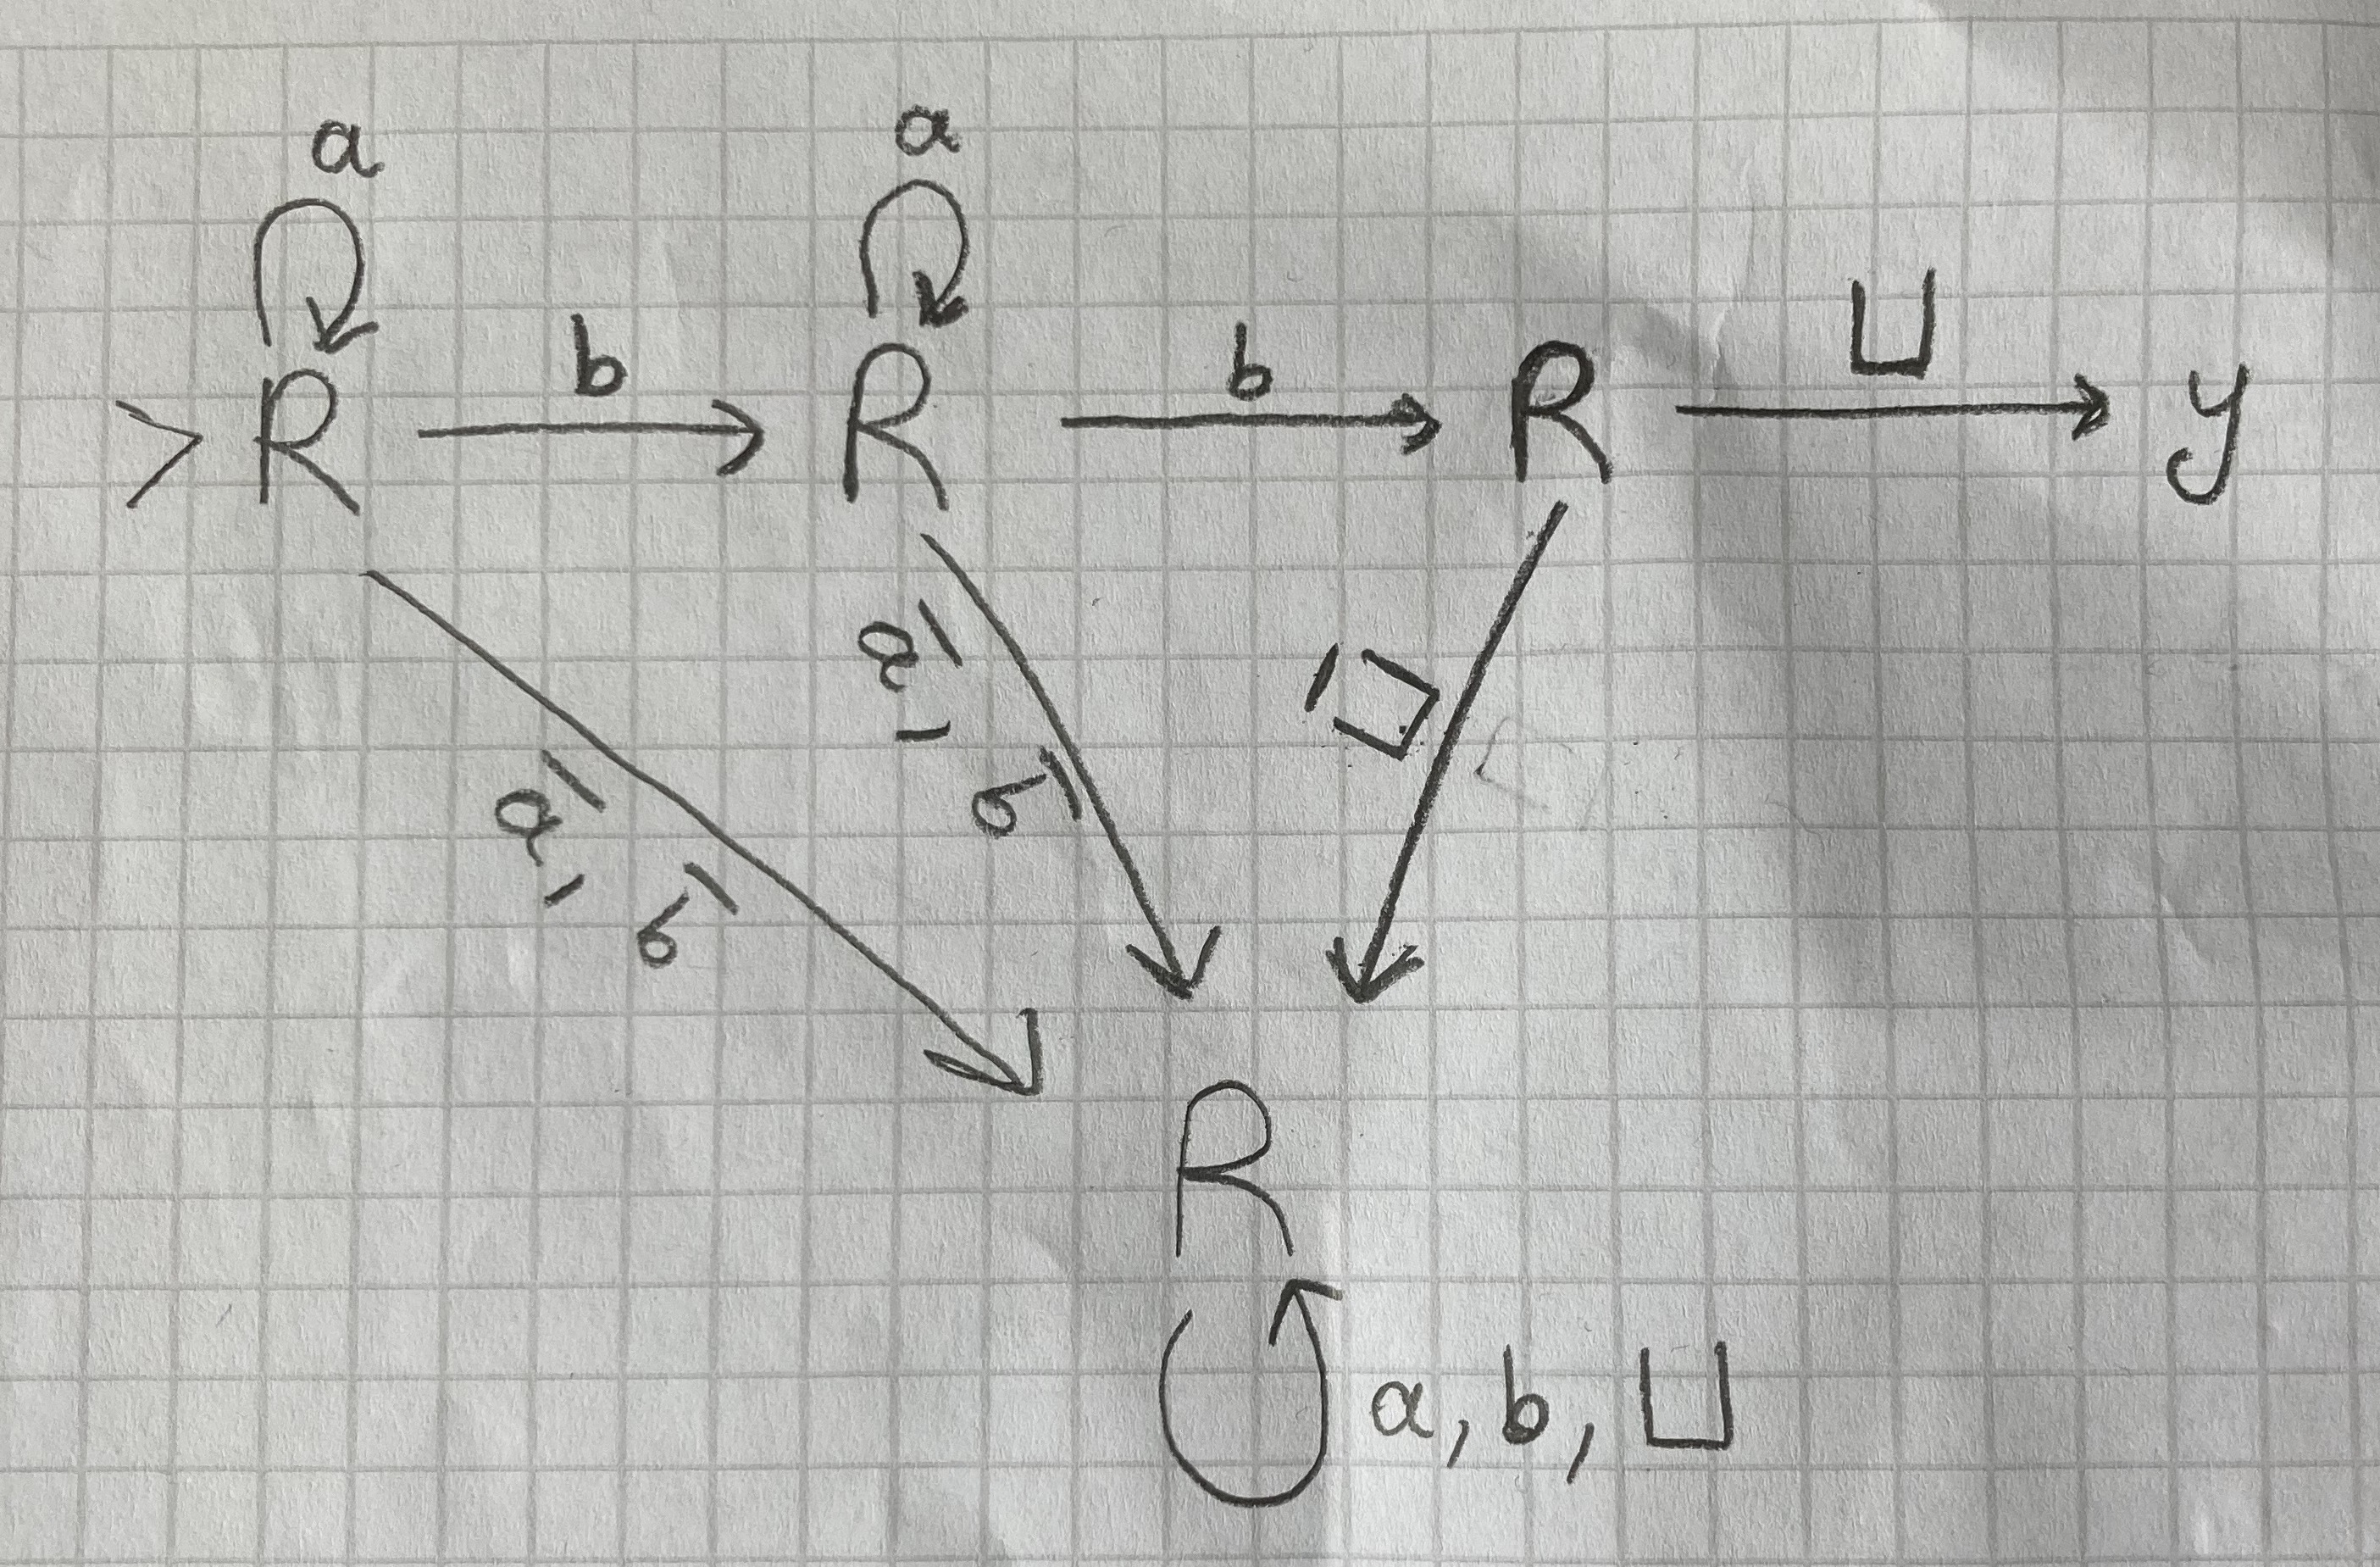
\includegraphics[width=1\textwidth]{IMG-0788.jpg} 

\section*{Answer 3}
1) Tape-1 takes $a$ and $b$ as input.\\
2) Copy $b$ to tape-2.\\
3) Write integer 1 to tape-3.\\
4) If the content of tape-2 is greater than zero; while it is greater than zero, multiply the content of tape-3 by $a$ (by calling $M_\times$) and decrement the content of tape-2 by 1 (by calling $M_-$). If the content of tape-2 is zero, the machine halts and outputs the content of tape-3.















\end{document}